\documentclass[border=4pt]{standalone}
\usepackage{mathptmx}
\usepackage{tikz}
\usetikzlibrary{positioning,arrows.meta}
\begin{document}
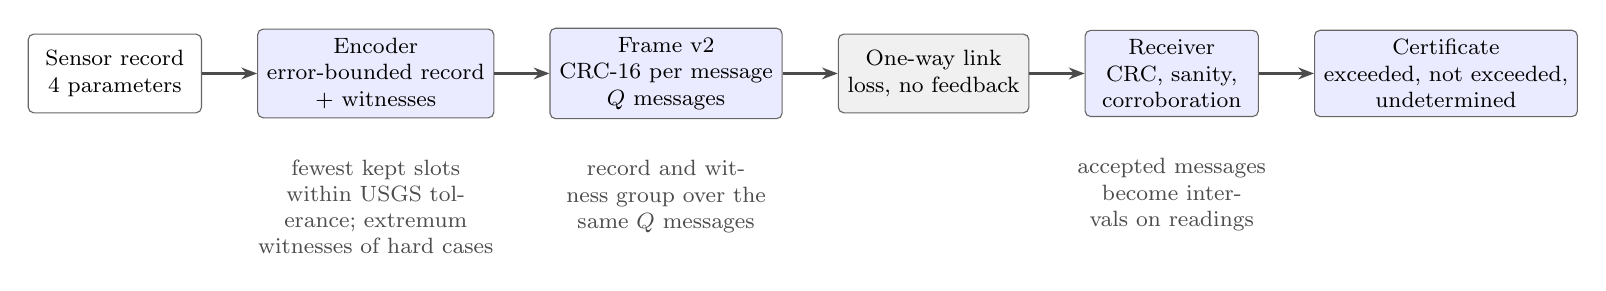
\begin{tikzpicture}[font=\footnotesize, node distance=5mm and 7mm,
  box/.style={draw=black!60, rounded corners=2pt, align=center, minimum height=10mm, minimum width=22mm, fill=white},
  hot/.style={box, fill=blue!8},
  arr/.style={-{Stealth[length=2mm]}, black!70, thick}]
  \node[box] (sensor) {Sensor record\\4 parameters};
  \node[hot, right=of sensor] (enc) {Encoder\\error-bounded record\\+ witnesses};
  \node[hot, right=of enc] (frame) {Frame v2\\CRC-16 per message\\$Q$ messages};
  \node[box, right=of frame, fill=black!6] (link) {One-way link\\loss, no feedback};
  \node[hot, right=of link] (rx) {Receiver\\CRC, sanity,\\corroboration};
  \node[hot, right=of rx] (cert) {Certificate\\exceeded, not exceeded,\\undetermined};
  \foreach \a/\b in {sensor/enc, enc/frame, frame/link, link/rx, rx/cert} \draw[arr] (\a) -- (\b);
  \node[below=4mm of enc, text width=3.2cm, align=center, black!70] {fewest kept slots within USGS tolerance; extremum witnesses of hard cases};
  \node[below=4mm of frame, text width=3.2cm, align=center, black!70] {record and witness group over the same $Q$ messages};
  \node[below=4mm of rx, text width=3.2cm, align=center, black!70] {accepted messages become intervals on readings};
\end{tikzpicture}
\end{document}
